\documentclass{article}
\usepackage[a4paper, total={6in, 8in}]{geometry}
\usepackage{stmaryrd} 
\usepackage{amssymb}
\usepackage{tikz}
\usetikzlibrary{positioning}

\title{Interaction Diagram - Remove Rating/Review}
\author{ Nicholas Riesen }

% no page number at bottom
\pagenumbering{gobble}

\begin{document}
\maketitle

\begin{center}

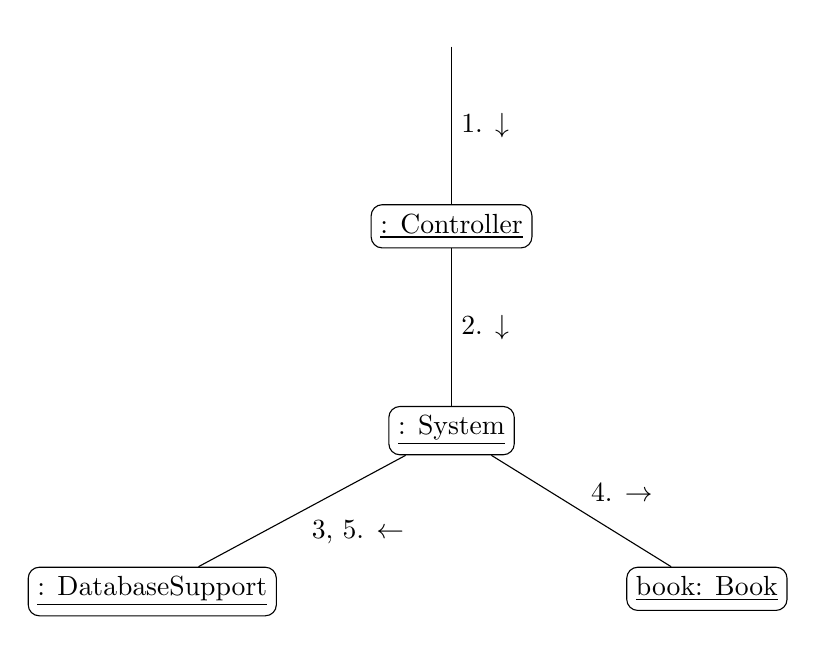
\begin{tikzpicture}[
  auto,
  block/.style = {
    rectangle,
    draw=black,
    align=center,
    rounded corners
  },
  multiple/.style = {
    rectangle, draw, rounded corners, fill= white,
    text width=9em, align= center,
    copy shadow = {
      ,fill=white, draw=black,
      shadow xshift=0.5mm, shadow yshift=-0.5mm
    }
  }
]
\node[] (start)  {};

\node[block, below = 2cm of start]           (controller) {\underline{: Controller}};
\node[block, below = 2cm of controller]      (system)     {\underline{: System}}; 
\node[block, below left = 2cm of system]     (database)   {\underline{: DatabaseSupport}};
\node[block, below right = 2cm of system]    (book)       {\underline{book: Book}};


\draw (start)      -- (controller) node[midway] {1. $\downarrow$};
\draw (controller) -- (system)     node[midway] {2. $\downarrow$};
\draw (system) -- (database)       node[midway] {3, 5. $\leftarrow$};
\draw (system)     -- (book)       node[midway] {4. $\rightarrow$};


\end{tikzpicture}

\vspace{0.5cm}

\begin{enumerate}
  \item b:= removeRateing(bid:String, reviewId:int):boolean
  \item b:= changeRateing(bid:String, reviewId:int):boolean
  \item book:= getBook(bid:String):Book
  \item b:= removeRateing(reviewId:int):boolean
  \item b:=putBook(book:Book):boolean
\end{enumerate}
\end{center}

\end{document}
